
\par\noindent\textit{引理~\ref{lem:7-2-285} 的证明（续）.}\quad
余下证明与第 7.2.9 小节的论证类似。
如下定义奇异单形集
$\mathcal X([0,1]^2\times L'_1)$：
其元素为满足
\[
\begin{aligned}
\operatorname{Eval}_{s=s_0}(\mathfrak P)
&\in C^{s=s_0}
([0,1]_r\times L'_1,(\lambda_0,\lambda'_1)),\\
\operatorname{Eval}_{r=r_0}(\mathfrak P)
&\in C^{r=r_0}
([0,1]_s\times L'_1,(\lambda_0,\lambda'_1))
\end{aligned}
\]
的奇异单形
$\mathfrak P\in S([0,1]^2\times L'_1)$。

首先考虑下式分解中出现的奇异单形：
\begin{equation}
\operatorname{Incl}_{1,\beta_0}(P)
\in S([0,1]^2\times L'_1).
\tag{7.2.296.1}\label{eq:7-2-296-1}
\end{equation}
其中 $P\in C(L'_1,\lambda'_1)$。
注意，$C(L'_1,\lambda'_1)$ 在此扮演
定义~\ref{def:7-2-188} 中 $C_0$ 的角色。
仿照定义~\ref{def:7-2-140}，再定义\translatornote{原书式 (7.2.296.2)
把双参数族写作 $\{\Phi_{s,t}\}_{s,t}$，
下文又称 $\psi_{r,s}$；情形 7.2.263
只定义了 $\Phi_{r,s}$，这里依该族及
引理 7.2.285 的同态记号统一为 $\Phi_{r,s}$。}
\begin{equation}
\{\Phi_{r,s}\}_{r,s*}(P)
\in S([0,1]^2\times L'_1).
\tag{7.2.296.2}\label{eq:7-2-296-2}
\end{equation}

从由 (7.2.296.1)、(7.2.296.2)
生成的 $S([0,1]^2\times L'_1)$ 子复形出发，
利用 (7.2.292.4) 添加奇异链，
使 (7.2.189.5) 成立。
随后，将前面得到的奇异单形分别与
带 $\operatorname{twp}(s)$、
$\operatorname{twp}(r)$ 条件的
伪全纯圆盘模空间作纤维积，
加入其三角剖分中出现的奇异单形。

下面说明可对所涉及的模空间选取三角剖分，
使所得链属于 $S_+([0,1]^2\times L'_1)$。
先把双参数族 $\Phi_{r,s}$ 重参数化，
使它在 $\partial[0,1]^2$ 附近
沿边界的法向方向保持常值；\translatornote{原书只说
“在 $\partial[0,1]^2$ 附近保持常值”，
但 (7.2.266) 指定的边界族可沿切向参数 $s$ 变化；
因此这里按与边界条件相容的法向局部常值理解。}
再选择扰动（多值截面），
使之在角点 $(s,r)=(s_0,r_0)$ 附近
沿离开角点的法向方向保持常值。
因此，在角点单形的附近，
可把模空间（即该纤维积）看作
包含于角点的单形与
$[0,\epsilon]\times[0,\epsilon]$ 的直积。
如同子引理~\ref{sublem:7-2-295} 的证明，
由此得到满足定义~\ref{def:7-2-288}
适配条件的单形。见图~\ref{fig:7-2-16}。

\par\medskip\noindent\begin{minipage}{\textwidth}
\centering
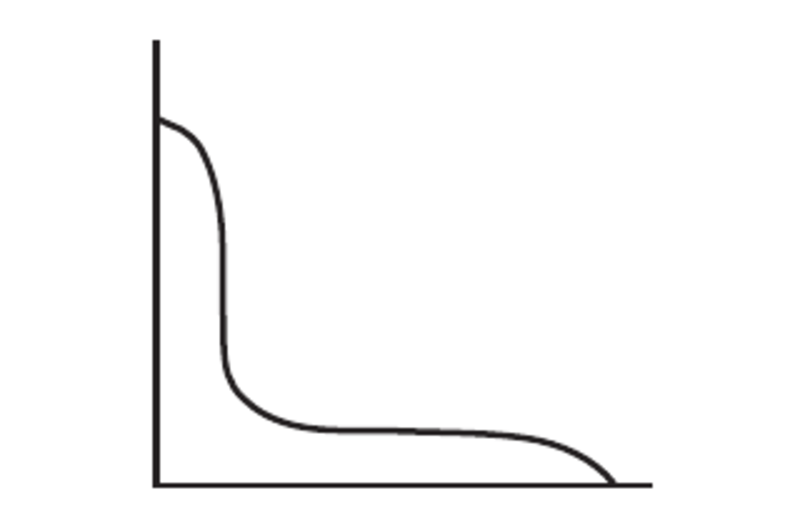
\includegraphics[width=.30\textwidth]{chapters/ch07-transversality/figures/phys-557-figure-7-2-16-math-crop.png}
\par{\renewcommand{\thefigure}{7.2.16}\refstepcounter{figure}
\normalfont\bfseries 图~\thefigure\label{fig:7-2-16}}
\end{minipage}\par\medskip

须注意，$S([0,1]^2\times L'_1)$ 中
可能有两条链 $\mathfrak P_1,\mathfrak P_2$，
其朴素交不满足 (7.2.289.3)。
例如，在 $[0,1]^2\times S^1$ 中取两个
二维单形 $\mathfrak P_1,\mathfrak P_2$，
使它们在 $[0,1]^2$ 上的投影
如图~\ref{fig:7-2-13}(1)。\translatornote{原书此处引作
“Figure 30.13 (1)”；本节相应的两幅三角形
实际编号为图 7.2.13(1)、(2)，故改引前者。}
容易找到一例，其交
$\mathfrak P_1\cap\mathfrak P_2$ 的投影
是连接 $(0,0)$ 与 $(\epsilon,\epsilon)$ 的线段。
还可使两单形的交横截，
且其维数为 $1=2+2-3$。
因此，朴素交
$\mathfrak P_1\cap\mathfrak P_2$
不满足 (7.2.289.3)。

不过，在这样的例子中，
$\mathfrak P_1$、$\mathfrak P_2$
在角点上的限制并不横截：
上述交在角点的预期维数是
$0+0-1=-1$，而非 $0$。
因此，表示交的运算 $\overline{\mathfrak m}_2$
已经过扰动，排除了这种现象。
处理好角点附近的横截性问题后，
余下构造与第 7.2.10 小节完全平行。

这样便构造出满足
(7.2.287.1)、(7.2.287.2) 的
映射 (7.2.286.1)、(7.2.286.3)。
为构造满足 (7.2.287.1) 的
映射 $\operatorname{Incl}_{k,\beta}$
（即 (7.2.286.2) 中的映射），
从 $\operatorname{Incl}_{1,\beta_0}$ 出发，
按归纳法定义 $\operatorname{Incl}_{k,\beta}$；
方法与命题~\ref{prop:7-2-162} 的证明相同。
引理~\ref{lem:7-2-285} 得证。$\square$
